
\section{User Interface}

It is the user interface (UI) that the user interacts with. The interface itself, as
shown in \autoref{fig:figure1}, is broken down into a number of separate areas:


\begin{figure}[!htbp]
  \centering {
    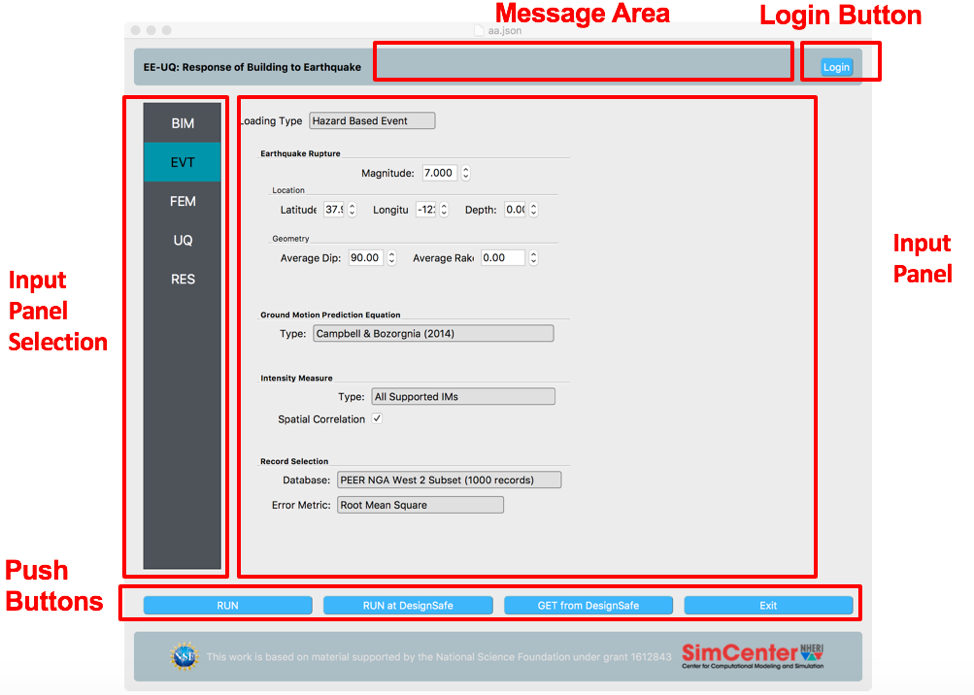
\includegraphics[width=0.8\textwidth]
    {figs/Figure1.png} }
  \caption{UI}
  \label{fig:figure1}
\end{figure}


\begin{enumerate}

\item Input Panel Selection: This  area on the left side provides the user with a selection of items to choose from from: 

\begin{enumerate}
  \item GI: General information, for specifiction of building description, location and units.
  \item SIM: Structure information model, for description of the building model.
  \item EVT: Event, for selecting the earthquake motions input.
  \item FEM: Finite element method, for specification of application and analysis options.
  \item UQ: Uncertainty quantification, for defining the distribution of the random
  variable paramaters and UQ method analysis options.
  \item EDP: Engineering demand parameters, for specification of output response quantities.
  \item RES: Results output.
\end{enumerate}

Selecting any of these will change the input panel presented.

\item Input Panel: This is the large central area of the UI that the user provides input
for the application chosen and views the results. For example if the user had selected UQ in the input panel selection, it is in this panel that the user would provide details on the distributions associated with each random variable or select the sampling method to use and provide the options necessary to run that method.

\item Push Buttons: This is the area near the bottom of the UI in which 4 buttons are presented to the user:

\begin{enumerate}
\item	RUN – to run the simulation of the user’s desktop machine.
\item	RUN at DesignSafe – to process the information, and send to DesignSafe where the job will be run on a supercomputer and results stored in your DesignSafe jobs folder.
\item	GET from DesignSafe – to obtain from DesignSafe your list of jobs and select from that list a job to download.
\item	Exit: to exit the application.
\end{enumerate}

The Screens presented to user when the first 3 of these buttons will be discussed in section 3.10.

\item Login Button: At the top right of the UI is the login button. Before the user can launch any jobs on DesignSafe they must first login to DesignSafe using their DesignSafe login and password. Pressing the login button will open up the login window for users to enter this information.

\item Message Area: In the top center of the application is the area of the interface that error and status messaged will be displayed while the application is running.

\end{enumerate}

\section{GI: General Information}
The user here provides information about the building and the units the user will work in. The widget itself presents 3 separate frames, as shown in \autoref{fig:figure2}, to the user:

\begin{enumerate}
\item Building Information frame in which user provide general information about the building, this include year of construction and type.
\item Properties frame in which user provides information about number of stories, width, depth, plan area and height of the building.
\item Location frame in which user provides location of the building. This information is used in some of event widgets to obtain events specific to the building.
\item Units frame  in which user specifies what the units will be for the inputs and outputs. Some widgets will require inputs in different units. These entries will contain units beside the specific entry to mark this.
\end{enumerate}


\begin{figure}[!htbp]
  \centering {
    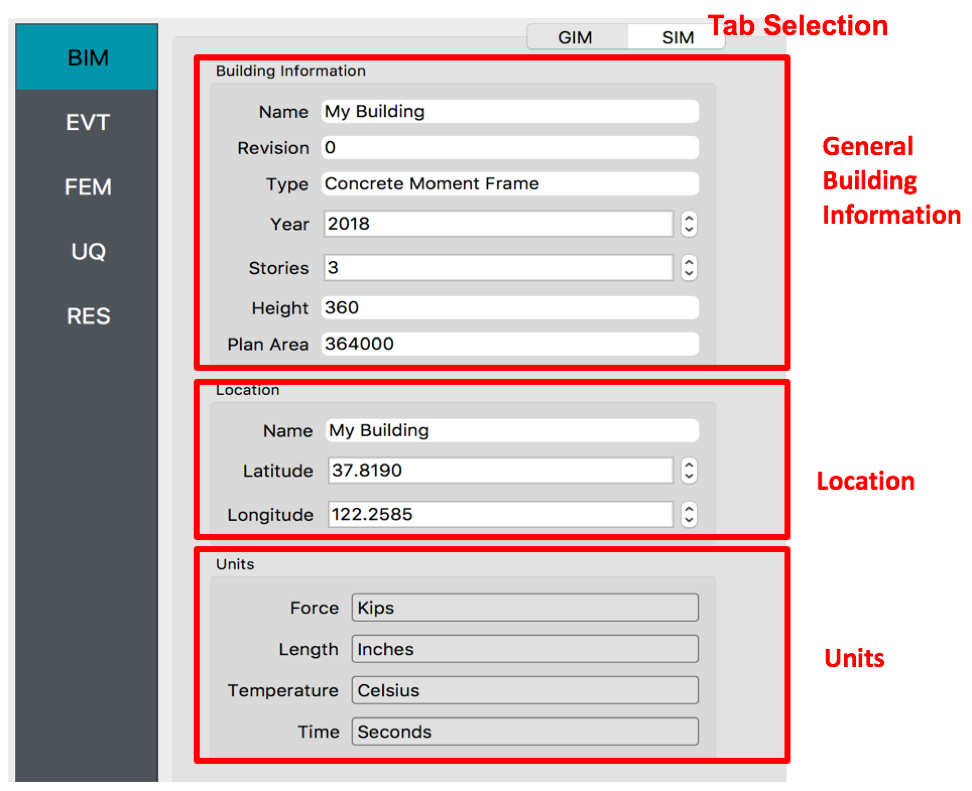
\includegraphics[width=0.8\textwidth]
    {figs/Figure2.png} }
  \caption{BIM}
  \label{fig:figure2}
\end{figure}

\section{SIM: Structural Information Model}

This panel is where the user defines the structural model of the building. The structural model is that part of the building provided to resist the lateral loads. There are a number of backend applications provided for this part of the workflow, each responsible for providing the structural analysis model to the workflow. The drop-down menu at the top of this panel is where the user selects which application to use. As the user switches between applications, the entry data changes to reflect the different inputs the different applications require. At present there are two backend applications available through the drop down menu: MDOF and OpenSees.

\subsection{MDOF}

This panel is provided for users to quickly create simple shear models of a building. The panel is divided into 3 frames:
\begin{enumerate}
\item in the top left frame the user enters the number of stories. For each story the user then enter the story height, initial stifness in 1 and 2 directions, yield strength in 1 and 2 directions, and hardeing ratio again in 1 and 2 directions. In addition user enters the floor weights and damping ratios for each of the modes.
\item In the lower left frame the user has the option of overriding an an individual floor or story basis, any of the properties set in the upper frame.
\item on the right side of the frame is a graphical widget showing the current building. When entering data into the lower left frame, those floors and stories corresponding to data being modified is highlighted in red.
\end{enumerate} 

Random Variables: Random Variables can be created by the user entering a valid string instead of a number in the entry fields for all entries except the number of floors. The variable name entered will appear as a Random Variable in the UQ panel and it is there that the user must enter the distribution for the Random Variable.


\subsection{OpenSees}
The panel is for users who have existing OpenSees model of a building that performs a gravity analysis and now wish to subject that building model to one of the EVENT options provided. The panel that presents is as shown in \autoref{fig:figure3}. The user has 3 fields that he needs to fill out:
\begin{enumerate} 
\item The user specifies the main script that contains the building model. This script should build a model and perform any gravity analysis of the building that is required before the event is applied.
\item A llist of nodes that define a column line of interest for which the responses will be determined. The column nodes should be in order from ground floor through to roof. The EDP options use this information to determine nodes at which displacement, acceleration and story drifts are calculated. 
\item An entry for the dimension of the model, i.e. 1D, 2D or 3D. This information is used to apply ground motions.
\end{enumerate}

\begin{figure}[!htbp]
  \centering {
    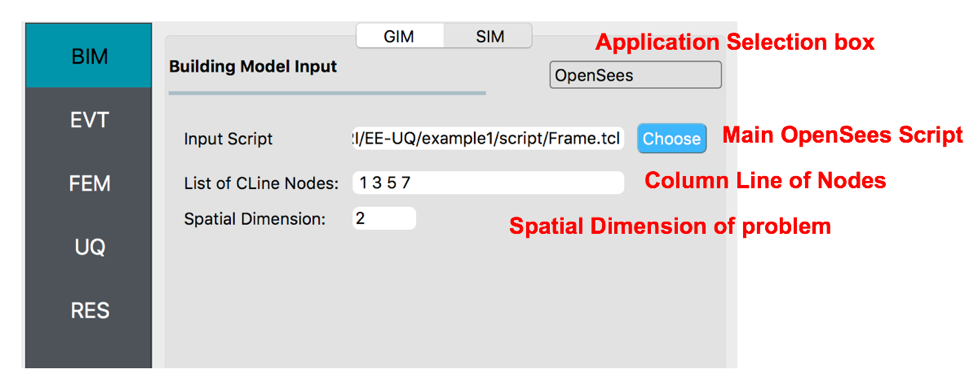
\includegraphics[width=0.8\textwidth]
    {figs/Figure3.png} }
  \caption{OpenSees Input Model}
  \label{fig:figure3}
\end{figure}

Random Variables: In OpenSees there is an option to set variables to have certain values using the pset command, e.g pset a 5.0 will set the variable a to have a value 5 in an OpenSees script. In EE-UQ any variable found in the main script to be set using the pset command will be assumed to be a Random Variable. As such, when a new main script is loaded all variables set with pset will appear as Random Variables in the UQ panel.


\section{EVT: Event}
The event panel presents the user with a drop-down menu with a list of available event applications. Event applications are applications that, given the building and user supplied data to the specific
applications input panel, will generate a list of events for the building. There are a number of options available in the pull-down menu.


\subsection{Multiple Existing}

This is provided for the user to specify multiple existing SimCenter
Event files.  If more than one event is specified it is done to provide
the UQ engine with a discrete set of events to choose from.  It is not
done with the intention of specifying that one event follows another.
The panel presented initially to the user is as shown
in \autoref{fig:figure4}.

\begin{figure}[!htbp]
  \centering {
    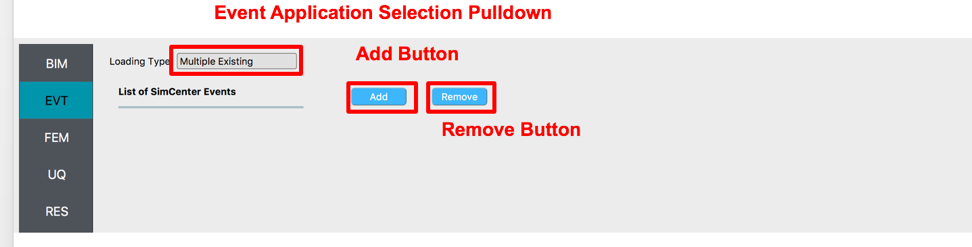
\includegraphics[width=0.8\textwidth]
    {figs/Figure4.png} }
  \caption{EVT}
  \label{fig:figure4}
\end{figure}

To add a new event, the user presses the Add button.  This adds an event to the panel.  Pressing the button multiple times will keep adding events to the panel.  \autoref{fig:figure5} shows the state after the button has been pressed twice, and data entered for the ElCentro and Rinaldi Events.

\begin{figure}[!htbp]
  \centering {
    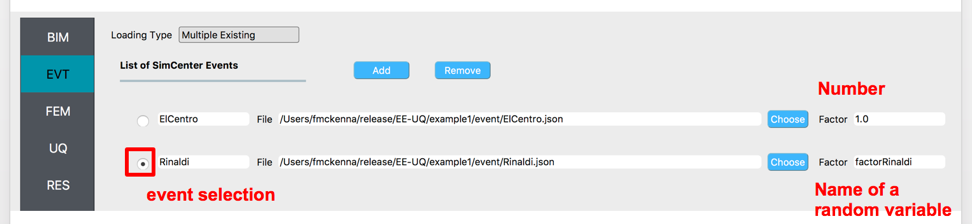
\includegraphics[width=0.8\textwidth]
    {figs/Figure5.png} }
  \caption{Adding new event}
  \label{fig:figure5}
\end{figure}


The user can enter the full path manually to the file or use the choose button,  which brings up your typical file search screen.  By default, a scaling factor of 1.0 is assigned to the event. 
The user can change this to another real value (AT PRESENT DO NOT USE INTEGER) or the user 
has the option of defining this to be a random variable by entering a name as shown for the second event. 

Note that this variable name must not start with a number, or contain any spaces or special characters, i.e. no -, +,..

The Remove button is pressed to remove events. To remove an event the user must first select
which events they wish to remove, done by clicking in the small circle at the start of the event. Once the events to remove  have been selected, the user removes all these selected evens by pressing the remove button.

If the user has multiple events to load, all the event files may first be placed by the user into a seperate folder. If the user presses the  Load Directory, the user will be able to choose a directory and the application will load all the event file (any file with a .json suffix) into the widget by choosing the directory. Initially each event will be given a load factor of 1.0.  Should the user include in that directory a file named Records.txt the application will open that file and load the events and assigned load factors from that file. Each line in Recors.txt is considered ro represent a record, and contains 2 comma seperated values: the first value being the event file and the second value the event factor. An example Records.txt is as shown below:

\begin{verbatim}
ElCentro.json,1.5
Rinaldi.json,2.0
\end{verbatim}

Random Variables: The user can, as mentioned, enter a string in the factor field to specify that the factor is to be considered a random variable. Subsequently in the UQ panel the user must provide information on the random variables distribution. Also, if multiple events are specified, the event itself will be treated as a random variable, with each event being part of the discrete set of possible events.

\subsection{Multiple PEER Event}
This is provided for the user to specify multiple existing PEER 
(\href{http://peer.berkeley.edu}{http://peer.berkeley.edu}) ground motion files. 
For PEER events the user is required to specify the individual components for the EVENTS. 
The Add/Remove buttons at the top are to create and remove an event, as per 2.2.1. 
For the PEER events the user specifies components acting in the individual degree-of-freedom directions. 
The + and – add and remove components with the remove removing all components selected. 
Each component in a PEER event can have their own scale factor, again a number or a random variable.

\begin{figure}[!htbp]
  \centering {
    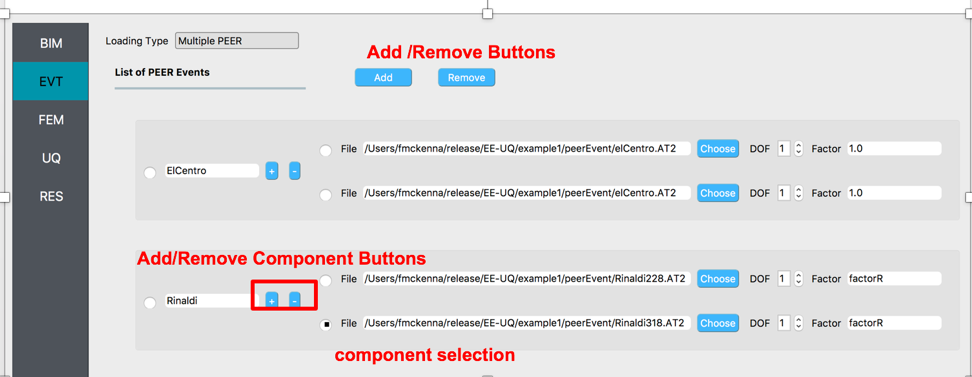
\includegraphics[width=0.8\textwidth]
    {figs/Figure6.png} }
  \caption{PEER event}
  \label{fig:figure6}
\end{figure}

If the user has multiple events to load the user can again place att the PEER .AT2 files into a separate folder and select the Load Directory option. This will allow the user to select a directory. Once selected all .AT2 files in that directory will be loaded into the application. Similar to loading multiple SimCenter events, should the user provide a file Records.txt in that directory, the application will load all files in the list and set the appropriate load factor. An example Results.txt file for multiple Peer events is as shown below:

\begin{verbatim}
elCentro.AT2,1.5
Rinaldi228.AT2,2.0
Rinaldi318.AT2,2.0
\end{verbatim}

Random Variables: The user can, as mentioned, enter a string in the factor field to specify that the factor is to be considered a random variable. Subsequently in the UQ panel the user must provide information on the random variables distribution. Also, if multiple events are specified, the event itself will be treated as a random variable, with each event being part of the discrete set of possible events.

\subsection{Hazard Based Event}
The panel for this event application is as shown
in \autoref{fig:figure7}.  This application implements a
scenario-based (deterministic) seismic event.  In this panel the user
specifies an earthquake rupture (location, geometry and magnitude), a
ground motion prediction equation, a record selection database and the
intensity measure used for record selection.  In the backend, this
application relies on three other applications to perform seismic
hazard analysis, intensity measures simulation (to create a simulated
target spectrum), and ground motion record selection/scaling.  Users
interested in learning about those applications are referred to the
documentation of the
(\href{https://github.com/NHERI-SimCenter/GroundMotionUtilities/blob/master/Readme.md}{SimCenter
ground motion utilities}).
\begin{figure}[!htbp]
  \centering {
    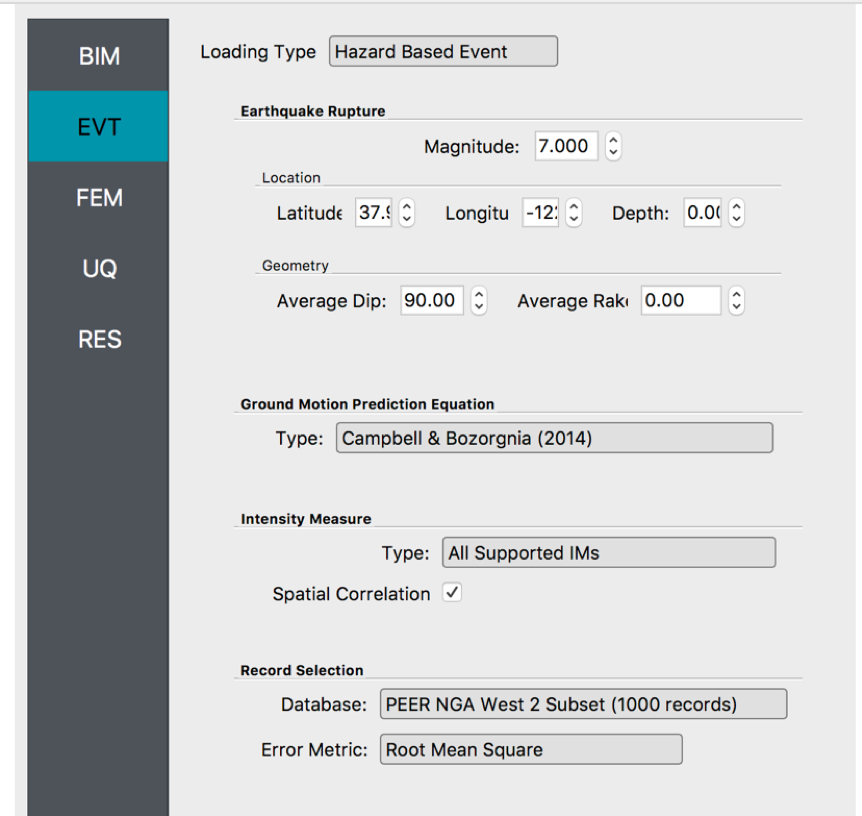
\includegraphics[width=0.8\textwidth]
    {figs/Figure7.png} }
  \caption{Hazard based event}
  \label{fig:figure7}
\end{figure}

\subsection{Stochastic Ground Motion Model}
This option allows users to generate synthetic ground motions for a
target seismic event. In order to do so, the stochastic ground motion
model is selected from the drop-down menu, as shown
in \Cref{fig:stochastic_loading}. Depending on the model selected, the
user will be asked to enter values for a number of parameters that are
used to generate a seismic event. In the current release, users can
select between the model derived by Vlachos et
al. (2018) \cite{vlachos2018predictive} and the model developed by
Dabaghi \& Der Kiureghian (2014, 2017, 2018)
[\cite{dabaghi2014stochastic}, \cite{dabaghi2017stochastic}, \cite{dabaghi2018simulation}]. Additionally,
users can provide a seed for the stochastic motion generation if they
desire the same suite of synthetic motions to be generated on multiple
occasions.  If the seed is not specified, a different realization of
the time history will be generated for each run. The backend
application that generates the stochastic ground motions relies
on \texttt{smelt}, a modular and extensible C++ library for generating
stochastic time histories. Users interested in learning more about the
implementation and design of
\texttt{smelt} are referred to its
\href{https://github.com/NHERI-SimCenter/smelt}{GitHub repository}.

All input parameters can be specified as random variables by entering
a string in the parameter field. Please note that information for the
inputs that are identified as random variables needs to be provided in
the \texttt{UQ} tab.

\begin{figure}[!htbp]
  \centering {
    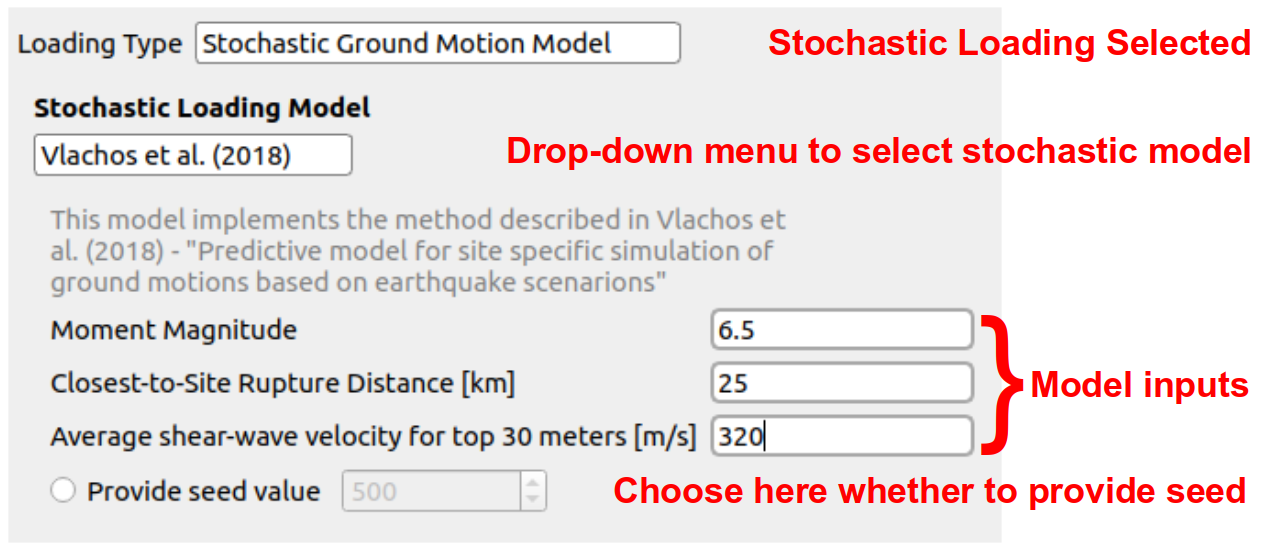
\includegraphics[width=0.8\textwidth]
    {usage/figures/stochastic_loading.png} }
  \caption{Stochastic Ground Motion Event}
  \label{fig:stochastic_loading}
\end{figure}




\subsubsection{s$^3$hark}
The panel for this event application is as shown in \autoref{fig:s3hark0}. 
This application does effective free-field site response analysis of a soil column.
In this panel the user specifies a ground motion at the bottom of the column. 
With soil layer properly defined, the motion at the ground surface will be given at the end of the analysis.
\begin{figure}[!htbp]
  \centering {
    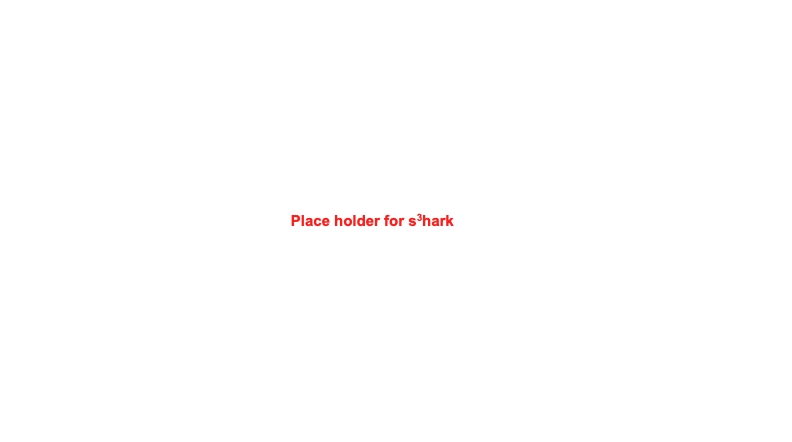
\includegraphics[width=0.8\textwidth]
    {figs/s3hark0.png} }
  \caption{s$^3$hark}
  \label{fig:s3hark0}
\end{figure}

The UI of s$^3$hark is shown in \autoref{fig:s3hark1}.
There are two graphics shown in the left of the panel. The first one is the soil column graphic, 
which shows a visualization of the soil column.
The second one is the mesh and profile graphic, 
which shows the finite element mesh and profile plots.
On the right of the panel are operation area, soil design table, configure tab, layer property tab and response tab. 


\begin{figure}[!htbp]
  \centering {
    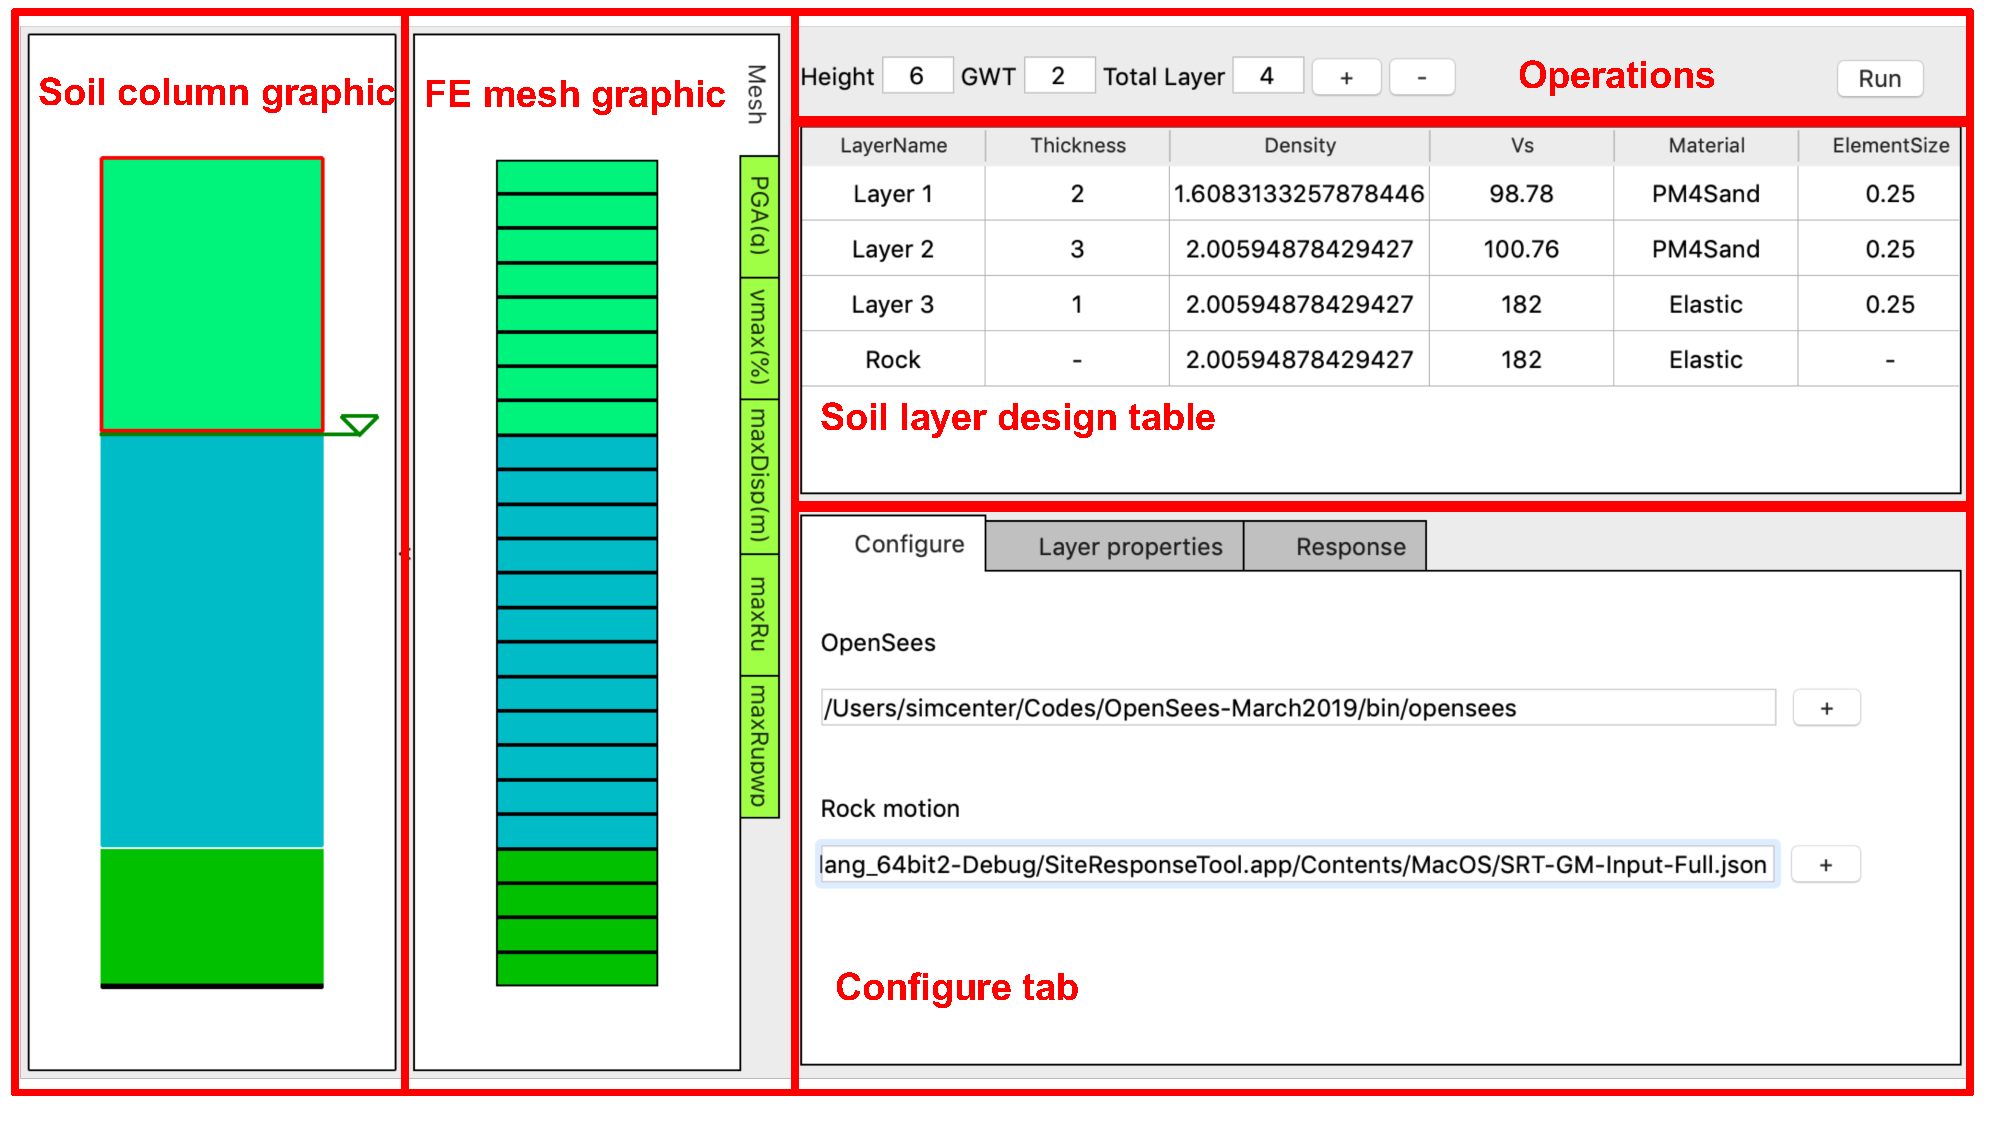
\includegraphics[width=0.8\textwidth]
    {figs/s3hark1.pdf} }
  \caption{s$^3$hark - Panels}
  \label{fig:s3hark1}
\end{figure}

In the operation area as shown in \autoref{fig:s3hark2}, click the plus button to add a layer and the minors button to delete a selected layer. 
Change the ground water table in the GWT input field. 
In the configure tab, path of OpenSees executable and rock motion file need to be specified.
A click on the run button will start the finite element analysis.


\begin{figure}[!htbp]
  \centering {
    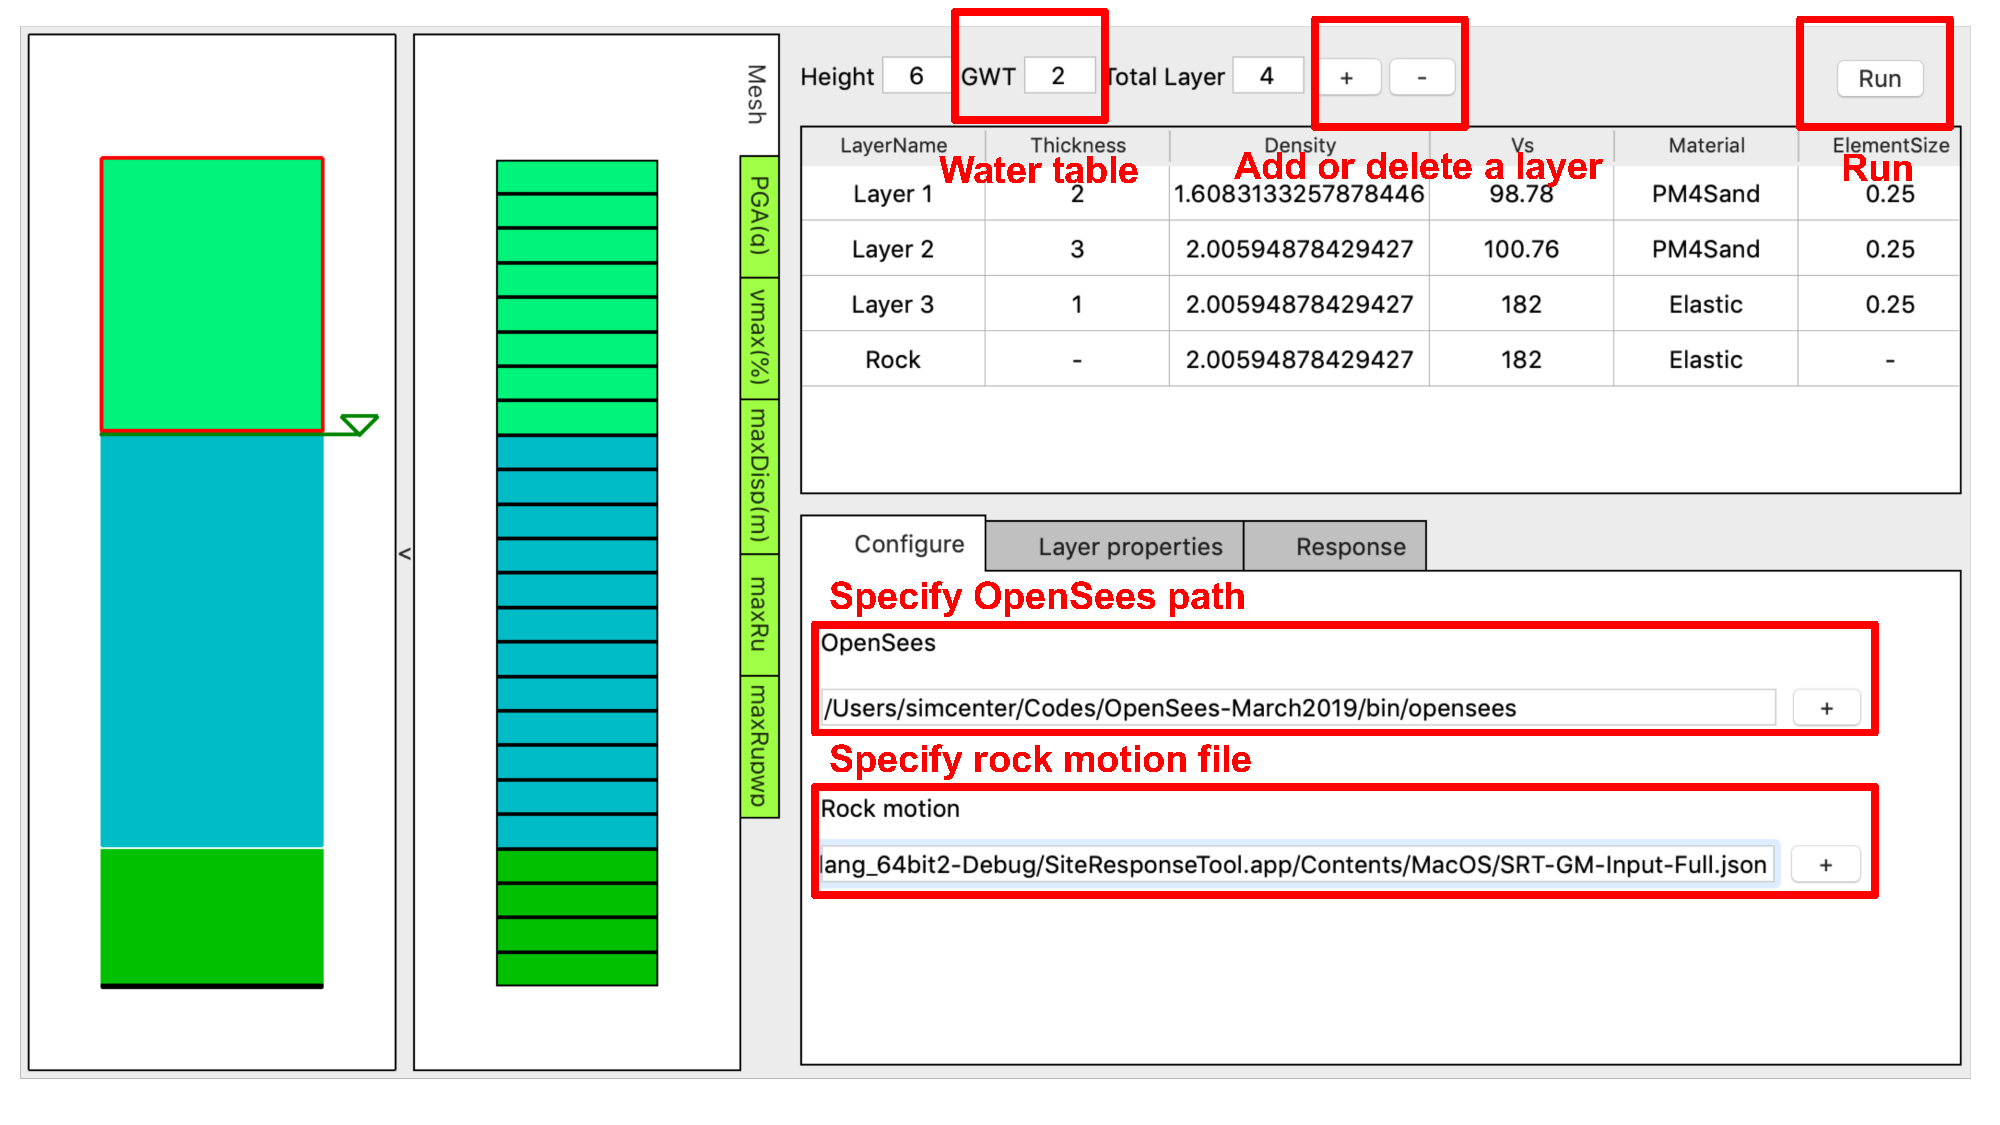
\includegraphics[width=0.8\textwidth]
    {figs/s3hark2.pdf} }
  \caption{s$^3$hark - Configurations and Operations }
  \label{fig:s3hark2}
\end{figure}

Either click on the soil column or the table to select a layer \autoref{fig:s3hark3}. 
When a layer is selected, it will be highlighted in both the soil column graphic and the table. 
Selection of a soil layer will invoke the Layer properties tab, where the user can specify the material properties of this layer.
Double click on a cell of the table will allow the user to change the corresponding value.

\begin{figure}[!htbp]
  \centering {
    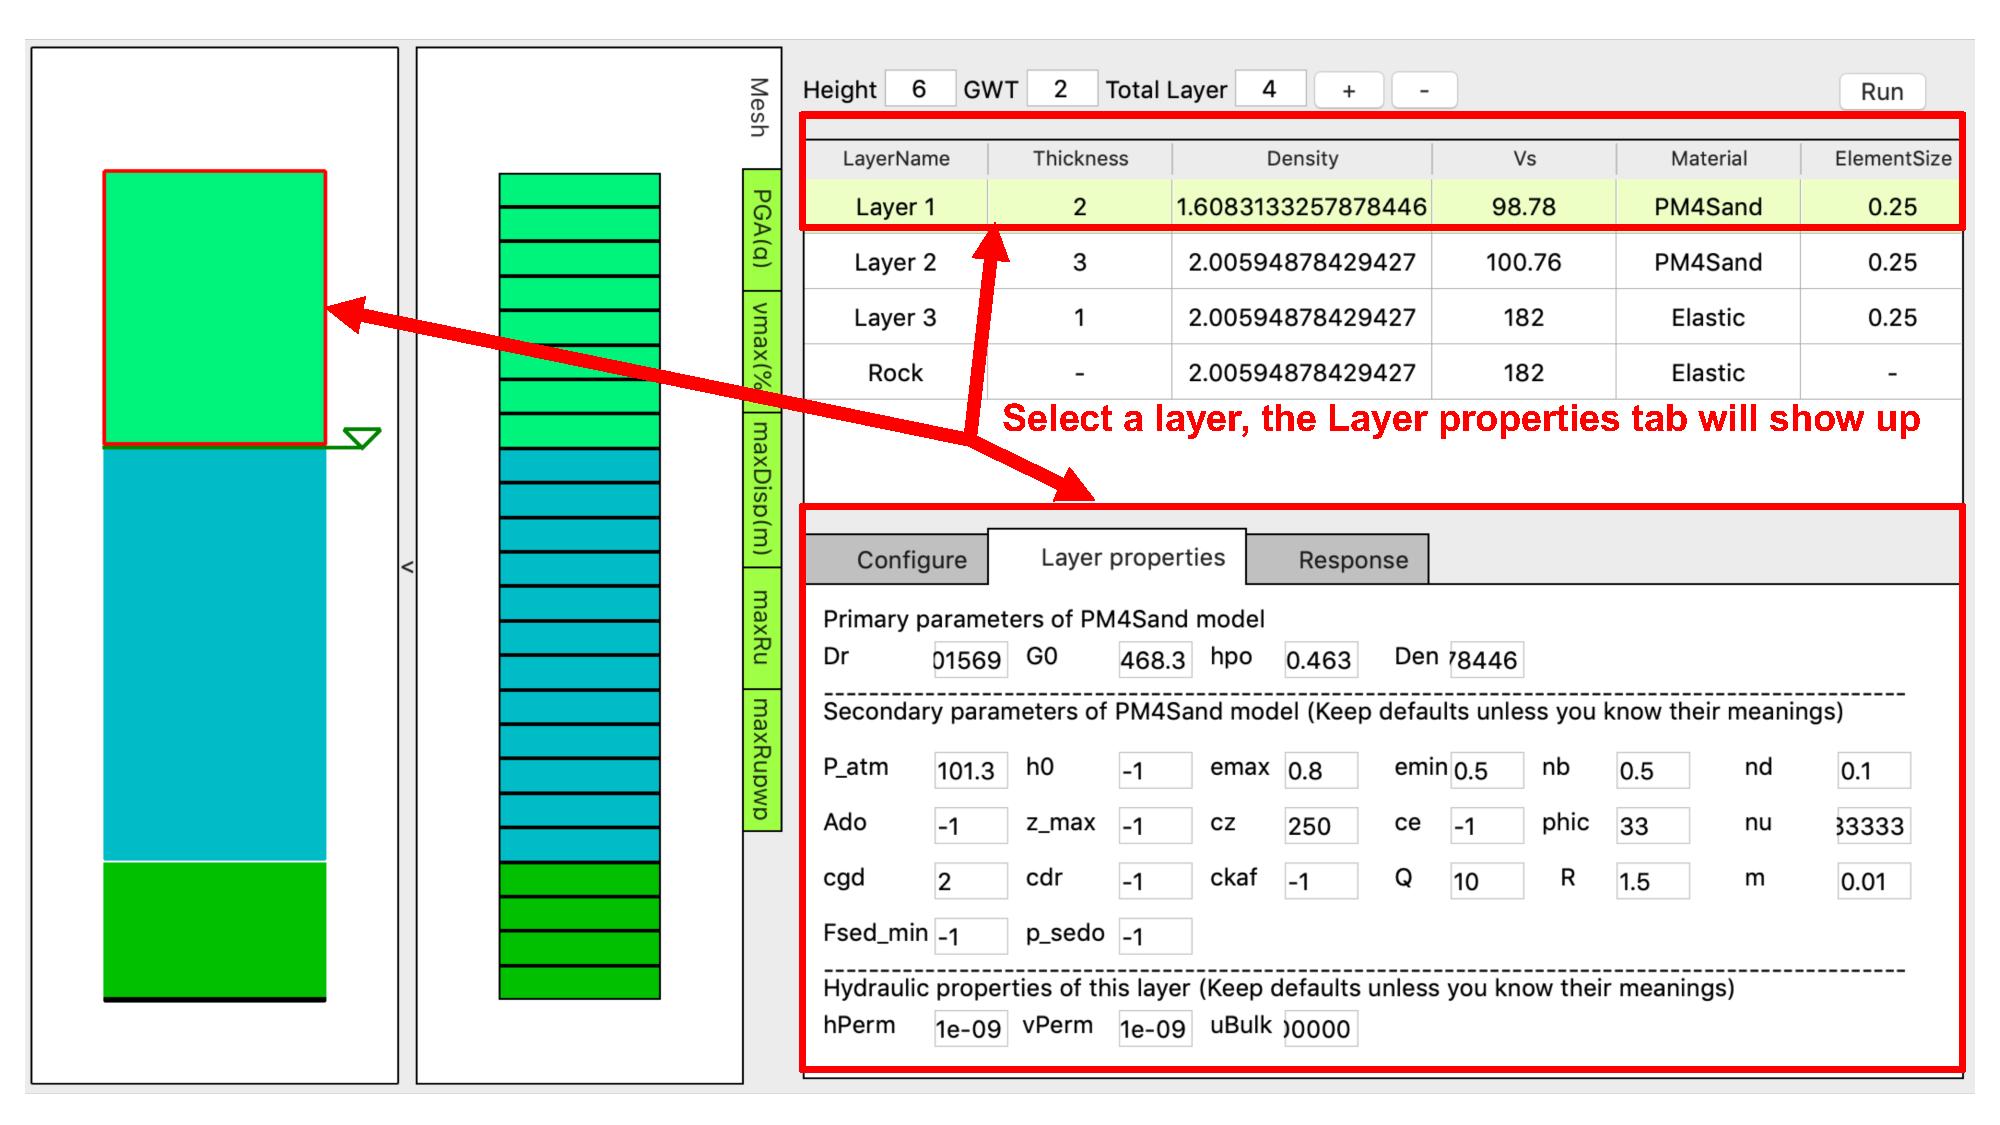
\includegraphics[width=0.8\textwidth]
    {figs/s3hark3.pdf} }
  \caption{s$^3$hark - Layer modification }
  \label{fig:s3hark3}
\end{figure}


Upon the finish of the finite element analysis, the ground motion at the soil surface (\autoref{fig:s3hark4}) will be stored in EE-UQ's input file.
This computed motion will be later applied to the bottom of the building.

\begin{figure}[!htbp]
  \centering {
    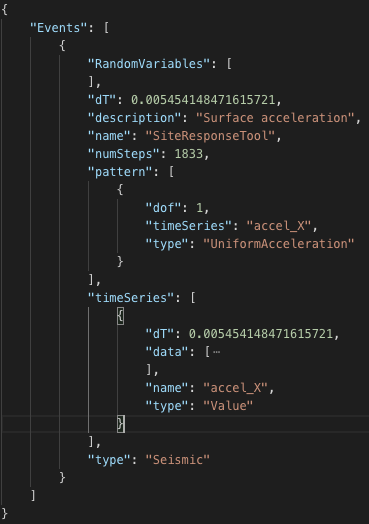
\includegraphics[width=0.4\textwidth]
    {figs/s3hark4.png} }
  \caption{s$^3$hark - Surface motion }
  \label{fig:s3hark4}
\end{figure}












\subsection{User Application}
The final selection option is a user specific application. 
The user specifies the application name and the input file containing the specific input information 
needed by the application when it is running in the backend. 
As will be discussed, the user is also required when they use an additional application not provided, 
to edit the tools registry file. Here they must include a new event application with this same name 
and the location where that application can be found relative to the tools application directory. 
If running on DesignSafe, that application must of course be built and available on the Stampeded2 supercomputer. 
NOTE that given how DesignSafe runs the applications through Agave, this applications file permissions must be 
world readable and executable (as when user running their application through DesignSafe and Agave, they are not running as themselves!)

\begin{figure}[!htbp]
  \centering {
    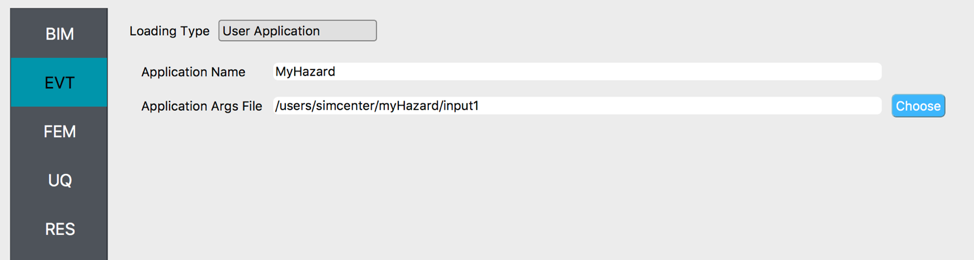
\includegraphics[width=0.8\textwidth]
    {figs/Figure8.png} }
  \caption{User defined event}
  \label{fig:figure8}
\end{figure}





\section{FEM: Finite Element Method}
The FEM panel is intended to present users with a selection of FEM applications that will take a building model generated by the BIM application and the EVENT from the event application and perform a deterministic simulation. 
At present there is only one application available, OpenSees and there is no application selection box.  That will be modified in future versionsto allow user to provide their own simulation application.  This is not the standard OpenSees executable, but consists of a pre- and post-processor to take the  BIM and EVENT file and use OpenSees to determine the response, returning these responses in an EDP. 

For the OpenSees application the user is required to specify the options to be used in the transient analysis. As shown in the figure this includes the choice of 
\begin{enumerate}
\item Solution algorithm, the default is Newton Raphson.
\item Integration Scheme, the default is Newmarks linear acceleration method.
\item Convergence Test, the default is a norm on the unbalance force.
\item Convergence tolerance
\item Damping Ratio.
\end{enumerate}

All the options available can be found in the OpenSees online user manual.\\

A default transient analysis script is run with these inputs. It is built for Version 3.0.0+ of OpenSees and uses a divide and conquer  algorithm in event of a convergence failure issue. This new algorithm does not always work. \\

The user is also able to specify their 
own analysis script to run instead of the default. When chosen the variables numStep and dt that are obtained from the EVENT are set by the program. These variables can be used by the user when providing their own analysis script.

\section{UQ}
Throughout the input specification the user is defining variables. As described in the above sections many of these variables can be specified by the user to be random variables with a distribution on their values. It is in the UQ panel that the user specifies what these distributions are. 
It is also here that the user specifies the UQ method and the input values are for these UQ methods. 
The panel is split,  as shown in \autoref{fig:figure10}, into 2 frames:
 \begin{enumerate}
\item Sampling Methods 
\item Random Variables
\end{enumerate}

\begin{figure}[!htbp]
  \centering {
    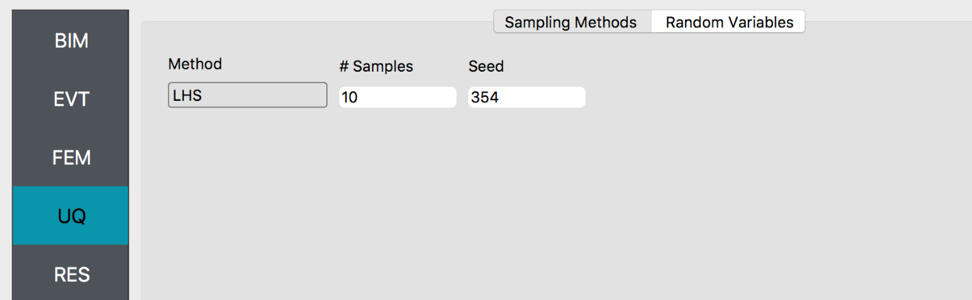
\includegraphics[width=0.8\textwidth]
    {figs/Figure10.png} }
  \caption{UQ}
  \label{fig:figure10}
\end{figure}


\subsection{Sampling Methods}
In the sampling methods the user selects the sampling method to use from the method dropdown. Currently this is limited to two options: 
Monte Carlo and Latin Hypercube Sampling (LHS). For the one selected, the user specifies the number of simulations to be perform and the seed.

\subsection{Random Variables}
The Random Variable panel is where the user enters the random variables. Each random variable has a name and a distribution. The distribution is selected frm the drop-down menu. By changing the distribution type, the inputs required to define the distribution change. The following are the list of distributions available:
\begin{enumerate}
\item Normal
\item Lognormal
\item Beta
\item Uniform
\item Weibull
|item Gumbell
\item UserDef
\end{enumerate} 

As with other panels, the random variables can be added or removed. Care must be taken by the user in ensuring that if the user removes random variables from this panel that they also remove them from the other input widgets. Failing to do so may result in the program faling to complete.


\begin{figure}[!htbp]
  \centering {
    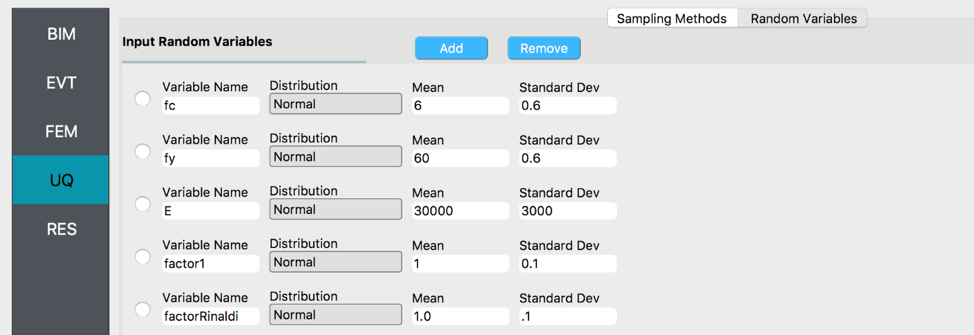
\includegraphics[width=0.8\textwidth]
    {figs/Figure11.png} }
  \caption{Random variables}
  \label{fig:figure11}
\end{figure}

\section{EDP: Engineering Demand Parameters}
This panel is where the user selects the outputs to be displayed when the simulation runs. There are two options available in the pull-down menu:
\begin{enumerate}
\item Standard Earthquake
\item USer Defined
\end{enumerate}

\subsection{Standard Earthquake}
When the user selects standard Earthquake there are no additional inputs required. The standard earthquake EDP generator will ensure the the max absolute value of the following are obtained: \begin{enumerate}
\item Relative Floor displacements:
\item Absolute Floor Accelerations
\item Interstory Drifts
\end{enumerate}

The  results will contain results for these in abbreviated form:
\begin{itemize}
\item PFD peak relative floor displacement $1-PFD-FLOOR_CLINE$
\item PFA peak floor acceleration (relative + ground motion): $1-PFA-FLOOR-CLINE$
\item PID peak inter-story drift: $1-PID-STORY-CLINE$
\end{itemize}

\subsection{User Defined}
This panel allows the user to provde to determine their own output and process it. When using this option the user provides additional data:
\begin{enumerate}
\item Additional Input: These are additional commands that are invoked by the analysis application before the transient analysis is performed. For example, foe OpenSees this would be a script containing a series of recorder commands.
\item Postprocess Script: This is a python script that will be invoked after the finite element application has run. It must be provided by the user. It's purpose is to process the output files and create a single file, results.out. This file must contain a single line with as many entries as EDP's specified.

\item Response Parameters. This is an area in which the user associates a variable name with the column of the results output file. If the process script has an array of strings named named EDP's the script, the Response Parameters will be initially set with these values from the script.
\end{enumerate}


\section{RES}

When the user hits the Run button, and assuming the results are successful. The results are presented here.  A successful run or download of a job that ran successfully will result in 3 tabbed widgets being displayed in this panel.  The first panel shows summary statistics: mean and stdDev values or min-max values if discrete set, i.e. multiple events for each of the EDP's specified in the EDP panel.

\begin{figure}[!htbp]
  \centering {
    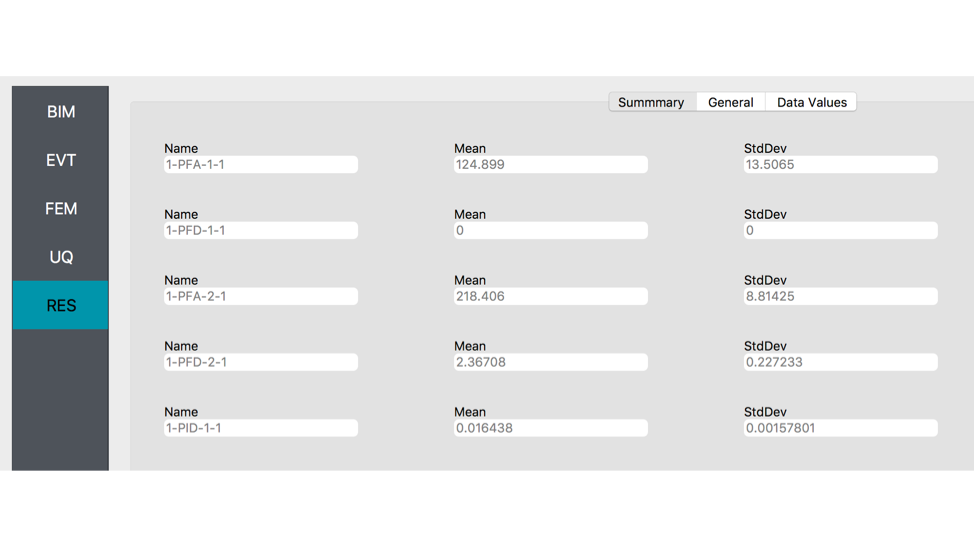
\includegraphics[width=0.8\textwidth]
    {figs/Figure12.png} }
  \caption{RES}
  \label{fig:figure12}
\end{figure}

The second panel shows the summary information.

\begin{figure}[!htbp]
  \centering {
    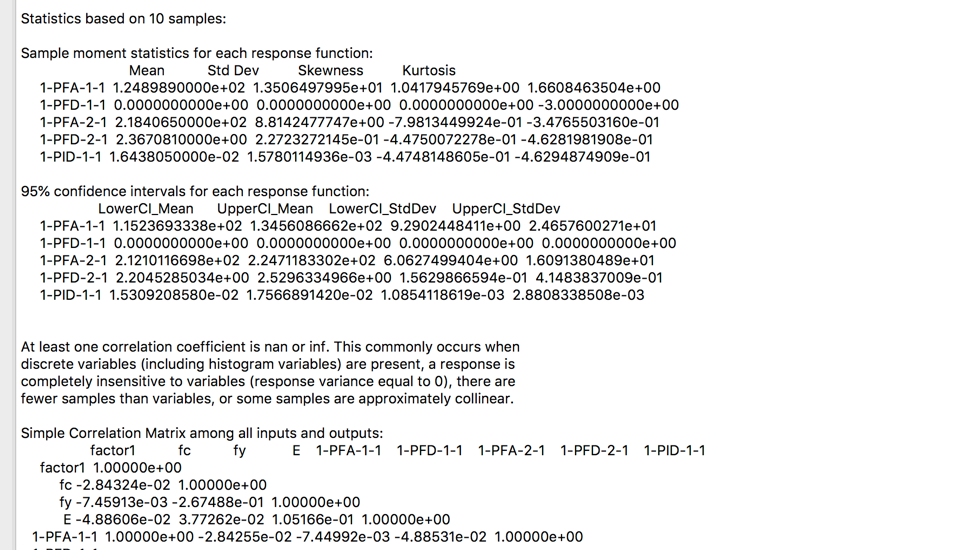
\includegraphics[width=0.8\textwidth]
    {figs/Figure13.png} }
  \caption{RES General tab}
  \label{fig:figure13}
\end{figure}

The third panel presents graphically and in tabular form the results. By selecting different columns with left and right mouse buttons in the table below the graphic, 
the information in the graph is changed. Selecting the left mouse button changes the Y axis, the right mouse changes the X axis. If the same column is selected 
using both left and right keys, the CDF and PDF is displayed. If last mouse press was with the left button, the PDF and if right the CDF.

As for the columns. You will see a column for each random variable the workflow came across. There may be more than you specified if the applications want the 
UQ engine to consider their own variables in the computation. The outputs at present are limited to:



\begin{figure}[!htbp]
  \centering {
    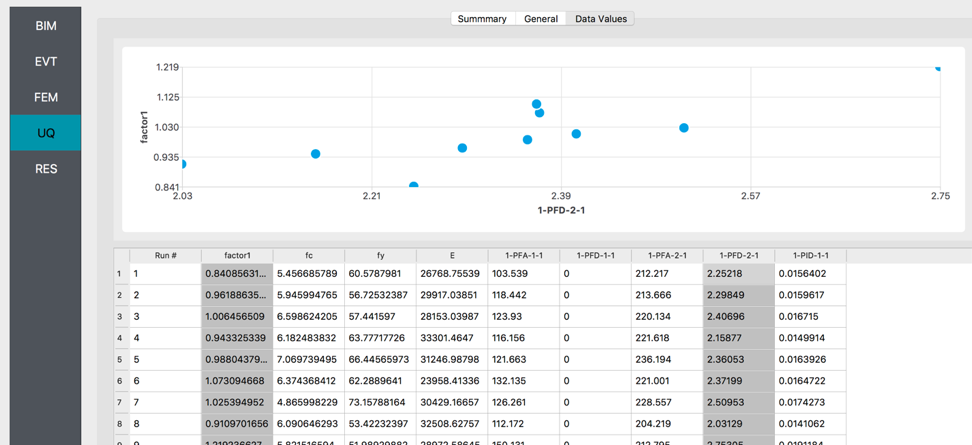
\includegraphics[width=0.8\textwidth]
    {figs/Figure14.png} }
  \caption{UQ Data Values}
  \label{fig:figure14}
\end{figure}



\section{Push Buttons}
There are a number of buttons in the Push Button area of \autoref{fig:figure1}:
\subsection{RUN – to run the simulation of the user’s desktop machine.}
\begin{figure}[!htbp]
  \centering {
    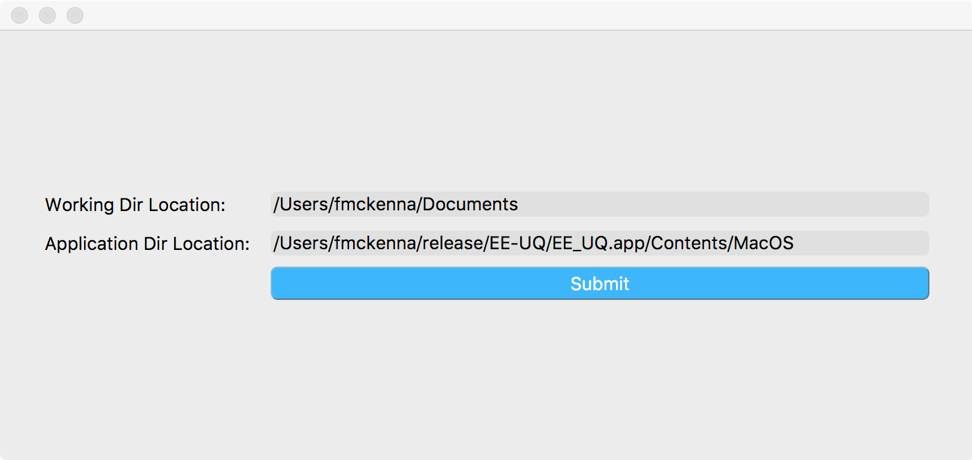
\includegraphics[width=0.8\textwidth]
    {figs/Figure15.png} }
  \caption{Run button}
  \label{fig:figure15}
\end{figure}
The window that pops up is as shown in \autoref{fig:figure15}. There are 2 entries and a push button: 

\begin{itemize}
\item Working Dir Location: specifies where the $EE_UQ$ application can create a “temporary” directory called tmp. SimCenter that the application 
creates when the submit button is pressed. The application creates this directory, copies files to it that the application needs as a result of your 
input (e.g. if you are using OpenSees input script, it will to the tmp. SimCenter directory copy that script, ALL FILES IN THAT DIRECTORY AND ALL FILES IN 
SUBDIRECTORIES OF THAT DIRECTORY GET COPIED SO DON’T PLACE THE SCRIPT IN HOME, DOWNLOADS, DOCUMENTS, ….
\item Application Dir Location: SHOULD NOT BE TOUCHED unless you are introducing your own applications or want to build and modify the 
applications provided with the tool. It is this directory the application tool looks to find the applications to run.
\end{itemize}


Finally, when inputs are finished the user hits submit button to start the backend job. If it runs the window will close and the RES 
panel will pop up on successful run. Do not press the submit button multiple times while waiting for it to close. We cannot guarantee 
what will happen and we did not disable the button in this release.

\subsection{RUN at DesignSafe}
Click this button to process the information, and send to DesignSafe where the job will be run on a supercomputer and results stored in your DesignSafe jobs folder.

\begin{figure}[!htbp]
  \centering {
    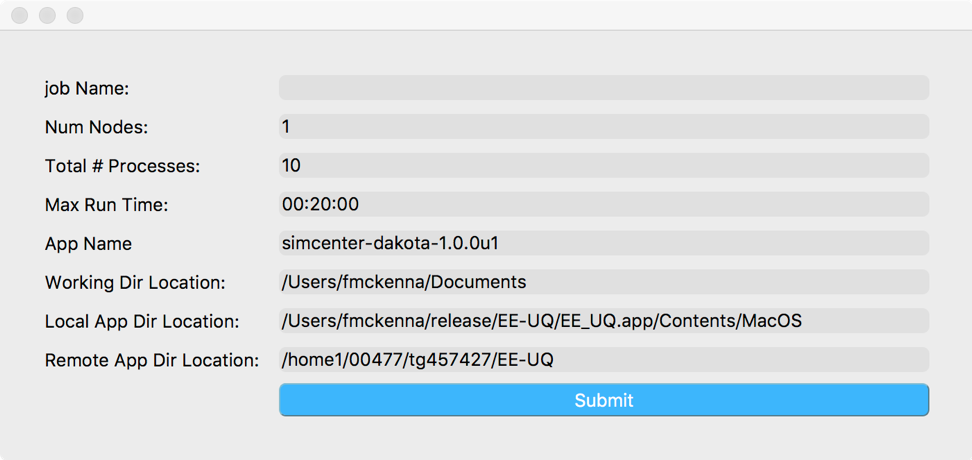
\includegraphics[width=0.8\textwidth]
    {figs/Figure16.png} }
  \caption{Remote button}
  \label{fig:figure16}
\end{figure}

A similar bit longer input panel is brought up:
\begin{itemize}
\item JobName: The name the user can use to identify the job in Get from DesignSafe.
\item NumNodes: The number of compute nodes to use on Stampede2. Using the default App Name the job will run on Stampede2’s KNL Landing (KNL) 
compute nodes. Each node has 68 cores. The actual number of cores the application will use on each of these nodes depends on the total number of 
processes specified. As per the TACC webpage, for MPI tasks it’s best not to specify more than 64-68 processes to run. Depending on the numerical 
computations and amount of memory each uses, so as to avoid page faulting, for large simulations you may wish to use more nodes and less processes.
\item Total Number of Processes: Total number of MPI parallel processes the UQ engine is going to use.
\item Max Wall Time:  HOURS:MIN:SEC be conservative. Your job is killed after the time limit. On Stampede2 you have a max wall time of 24 hours.
\item App Name:   Name of Agave app to run. DO not touch unless you know what you are doing.
\item Working Dir Location: specifies where the $EE_UQ$ application can create a “temporary” directory called tmp. SimCenter that the application 
creates when the submit button is pressed. The application creates this directory, copies files to it that the application needs as a result of your 
input (e.g. if you are using OpenSees input script, it will to the tmp. SimCenter directory copy that script, ALL FILES IN THAT DIRECTORY AND ALL FILES 
IN SUBDIRECTORIES OF THAT DIRECTORY. (SO, DON’T PLACE THE SCRIPT IN HOME, DOWNLOADS, DOCUMENTS, …). That directory is removed when jib has been successfully submitted.
\item Local App Dir Location: SHOULD NOT BE TOUCHED unless you are introducing your own applications or want to build and modify the applications 
provided with the tool. It is this directory the application tool looks to find the applications it needs.
\item Remote App Dir Location: Remote directory on Stampede2 where applications needed by workflow reside. DO not touch unless you know what you are doing.

\end{itemize}


\subsection{GET from DesignSafe}
	Click this button to obtain from DesignSafe your list of jobs and select from that list a job to update status of, download or delete.

\subsection{Exit}
Click this button to exit the application. 
